The following lab materials are provided: 

\begin{enumerate}
	\item 2 plastic cups 
	\item 6 baffles: 2 Rushton, 2 Pitched-blade, 2 Paddle 
	\item Magnetic Stirrer and plate 
	\item Shaft and lid  
	\item Blue dye 
\end{enumerate}

%\begin{figure}[h]
%	\begin{minipage}{0.33\textwidth}
%		\includegraphics[]{}
%		\caption{Pitch-blade Impeller}
%	\end{minipage}
%	\begin{minipage}{0.33\textwidth}
%		\includegraphics[]{}
%		\caption{Paddle Impeller}
%	\end{minipage}
%	\begin{minipage}{0.33\textwidth}
%	\includegraphics[]{}
%	\caption{Rushton Impeller}
%\end{minipage}
%\label{fig:}
%\caption{Type of impellers that are used in this experiment \cite{Altman1998}
%\end{figure}

Four comparative experiments were designed to investigate the optimal bioreactor prototype by considering the following aspects: 
\begin{enumerate}
	\item Which one of the three types of impellers is the most efficient? In this experiment, individual impellers of each type were assessed on its mixing time over various rotational speed, starting from 60rpm. For each impeller, mixing time is plotted against rotational speed. The rotational speed giving the least time is the optimal rotational speed. The impeller that achieves mixing under the least time and least rotational speed is the optimal choice.
	\item Do baffles assist mixing? This element was tested using Rushton under baffled versus unbaffled conditions. To test whether baffles are helpful, both conditions are tested under the optimal rotational speed, 280rpm. Whichever condition with the less mixing time is the preferred.
	\item Do multiple impellers work better than a one? 2 Rushton turbines were tested for rotational speeds 260rpm, 280rpm, and 300rpm. The mixing time under each speed is compared to that for 1 Rushton turbine.
	\item If using two impellers, which combination is the most efficient? From experiment one, the least efficient impeller can be eliminated. Thus, in this experiment, different combinations of the most efficient impeller types will be assessed for various rational speed.
\end{enumerate}

Procedures of the experiments are described in detail as follows: 
\begin{enumerate}
	\item Assemble the impeller of choice with the shaft, stirrer, and mixing vessel. 
	\item Add 300mL of water to the vessel. 
	\item Put the vessel on the magnetic plate. 
	\item Adjust the rotational speed to the one of choice and wait until the number blinks on the display panel suggesting that the desired speed is achieved. 
	\item Add 5 drops of blue dye at 2cm from the top of the cup to the water. Must keep the height at 2cm each time to ensure consistency throughout the experiment.  
	\item Start the timer when the first drop is added; stop the timer when the color is evenly distributed in water. 
	\item Repeat 1-6 for different settings including different types of impellers, various rotational speeds, baffled versus unbaffled conditions, and different numbers of impellers. Specific set up is determined by the four comparative experiments mentioned above.  
\end{enumerate}

\begin{figure}[h]
	\centering
	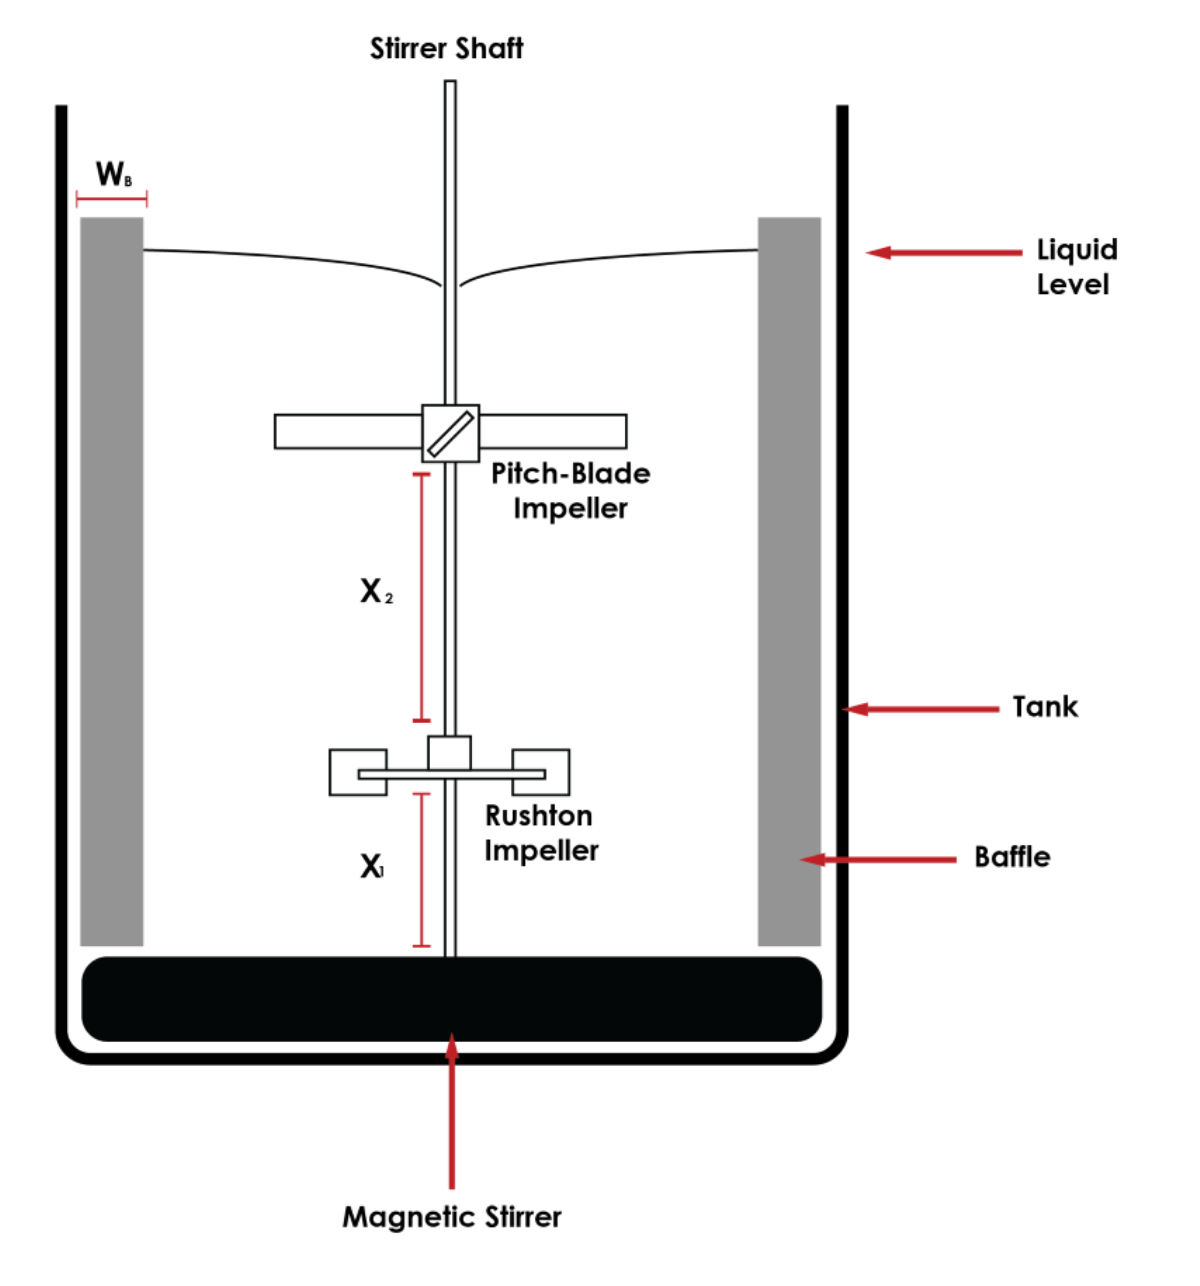
\includegraphics[width=0.4\textwidth]{Stirrer.png}
	\caption{bench scale reactor prototype layout}
\end{figure}








